\documentclass[a4paper,12pt,oneside]{book} % nie: report!


% pakiety
\usepackage{polski} % lepiej to zamiast babel!
\usepackage[utf8]{inputenc} % w razie kłopotów spróbować: \usepackage[utf8x]{inputenc}
\usepackage{fancyhdr} % nagłówki i stopki
\usepackage{indentfirst} % WAŻNE, MA BYĆ!
\usepackage[pdftex]{graphicx} % to do wstawiania rysunków
\usepackage{amsmath} % to do dodatkowych symboli, przydatne
\usepackage[pdftex,
            left=1in,right=1in,
            top=1in,bottom=1in]{geometry} % marginsy
\usepackage{amssymb} % to też do dodatkowych symboli, też przydatne
\usepackage{pdfpages}
\usepackage{lipsum}
\usepackage{multirow}
\usepackage{listings}
\usepackage{caption}
\usepackage{booktabs}
\graphicspath{ {./img/} }
\DeclareCaptionType{code}[Listing][Spis listingów] 

% definicje nagłówków i stopek
\pagestyle{fancy}
\renewcommand{\chaptermark}[1]{\markboth{#1}{}}
\renewcommand{\sectionmark}[1]{\markright{\thesection\ #1}}
\fancyhf{}
\fancyhead[LE,RO]{\footnotesize\bfseries\thepage}
\fancyhead[LO]{\footnotesize\rightmark}
\fancyhead[RE]{\footnotesize\leftmark}
\renewcommand{\headrulewidth}{0.5pt}
\renewcommand{\footrulewidth}{0pt}
\addtolength{\headheight}{1.5pt}
\fancypagestyle{plain}{\fancyhead{}\cfoot{\footnotesize\bfseries\thepage}\renewcommand{\headrulewidth}{0pt}}


% interlinia
\linespread{1.25}


% treść
\begin{document}
\sloppy
\thispagestyle{empty}

\includepdf{stronatytulowa}
\newpage{}

\thispagestyle{empty}
\newpage{}

\tableofcontents{}

\chapter*{Wstęp}
\addcontentsline{toc}{chapter}{Wstęp}
\label{Wstep}
%Mega ogólne sprawy dotyczące tego co chce zrobić
Sieci neuronowe mają za zadanie naśladowanie zachowań sieci neuronów znajdujących się w mózgu człowieka. Zostały stworzone do rozwiązywania zadań trudnych lub prawie niemożliwych do opisania za pomocą reguł, wyrażeń logicznych i innych narzędzi programistycznych. Wraz z rozwojem sieci neuronowych powstało wiele wariantów, które ze względu na swoją budowę lepiej lub gorzej sprawdzają się w różnych problemach. W przypadku rozpoznawania obrazów w postaci dwu-wymiarowej macierzy dla danych monochromatycznych lub trój-wymiarowej macierzy dla zdjęć kolorowych jednym z najlepszych wyborów będą sieci konwolucyjne. Sieci te rozpoznają wzorce, poczynając od linii horyzontalnych i wertykalnych, a w dalszych warstwach kończąc na skomplikowanych strukturach. Budowa i działanie sieci konwolucyjnych daje wielki potencjał do klasyfikacji obrazów. Ta praca przedstawi przykład takiej klasyfikacji wieloklasowej z użyciem sieci konwolucyjnych na przykładzie alfabetu Amerykańskiego Języka Migowego. 

\chapter*{Cel i zakres pracy}
\addcontentsline{toc}{chapter}{Cel i zakres pracy}
\label{Cel i zakres pracy}
%celem pracy jest napisanie programu bla bla
Celem pracy jest stworzenie programu wyposażonego w wytrenowany model do rozpoznawania obrazu, który w czasie rzeczywistym używając kamery internetowej będzie w stanie odczytać i wyświetlić na ekranie transkrypcję znaków języka migowego pokazywanych przez osobę znajdującą się w polu widzenia kamery. Dodatkowo do pracy będą składać się: utworzenie zbioru danych składającego się z około 50000 zdjęć zawierających wszystkie litery alfabetu ASL, utworzenie modelu z warstw konwolucyjnych i gęstych oraz wytrenowanie modelu i tuning parametrów. W części teoretycznej pracy zostanie przybliżony temat języka migowego American Sign Language, jak również temat konwolucyjnych sieci neuronowych i sposobu działania modeli.

\chapter{Język migowy American Sign Language}
American Sign Language (Amerykański Język Migowy, ASL) to złożony język wizualno-przestrzenny używany przez ludzi głuchoniemych w Stanach Zjednoczonych Ameryki oraz anglojęzycznych częściach Kanady. Jest to w pełni kompletny język naturalny. ASL jest językiem natywnym dla wielu głuchoniemych mężczyzn, kobiet i dzieci, a także niektórych słyszących dzieci w rodzinach, gdzie opiekunowie prawni są niesłyszący.\cite{nakamura}
\section{Historia}
Pochodzenie dzisiejszej społeczności osób głuchoniemych w Stanach Zjednoczonych jest powszechnie utożsamiane z założeniem pierwszej szkoły dla niesłyszących - American School for the Deaf (ASD), założonej w 1817 roku w Hartford, Connecticut. Przed założeniem szkoły ASD na terenie USA działało wiele niezależnych społeczności, poczynając od małych grup o wielkości pojedynczej rodziny do większych - całych wsi. W małych społecznościach uformowały się niezależne znaki i systemy języka migowego, które są obecne po dziś dzień w tych środowiskach. Istnieją dowody na to, że głuchonieme dzieci kształtowały swoje własne systemy języków migowych, które były o wiele bardziej wyrafinowane od tych, używanych w społeczności, w których się znajdowały.\cite{bahan}

Istnieją również doniesienia o innym niezależnie uformowanym systemie języka migowego Martha’s Vineyard Sign Language (MVSL), który istniał przed założeniem American School for the Deaf. Język ten był głównie używany w wsi Chilmark na wybrzeżu Massachusetts. Powstanie MVSL zapoczątkował fakt, że wspomniana społeczność Chilmark miała wysoki odsetek mutacji genetycznych prowadzących do głuchoty. W skali miasteczka około 4 procent mieszkańców było głuchoniemych. Wynikało to z wysokiego odsetka mieszanych małżeństw od wielu pokoleń, począwszy od hrabstwa Kent w Angli, zanim wieś Chilmark została założona w roku 1690.\cite{groce} Mieszkańcy, którzy nie byli głuchoniemi również posługiwali się językiem MVSL, wówczas gdy znajdowali się w towarzystwie osób z niepełnosprawnością ale również, gdy w gronie rozmówców nie było osoby głuchoniemej. Język był używany do czasu założenia szkoły dla osób głuchoniemych ASD w Hartford. Dzieci z wsi Chilmark zaczęto wysyłać do szkoły American School for the Deaf we wczesnych latach dwudziestych XIX wieku. Skutkowało to zatarciem się języków MVSL i nowego języka migowego ewoluującego w dzisiejszy język ASL.\cite{bahan}

Kiedy szkoła dla głuchoniemych została założona, stała się miejscem, gdzie wiele pomniejszych systemów migowych stykało i mieszało się ze sobą przez 175 lat. Z mieszanki tych języków powstał dzisiejszy język ASL. Głuchoniemy nauczyciel - Laurent Clerc, pochodzący z Francji, był pierwszym nauczycielem w wspomnianej placówce. Z kraju swojego pochodzenia przywiózł wiedzę o Francuskim Języku Migowym, którego znaków nauczał w amerykańskiej szkole. Ta sytuacja spowodowała bardzo mocne doprawienie wówczas powstającego języka ASL o aspekty zaciągnięte z Francuskiego Języka Migowego. Na dzień dzisiejszy około 60 procent współczesnego systemu ASL opiera się na starym migowym języku Francuskim.\cite{bahan}


\section{Populacja}
Informacje dostępne w internecie nie dają jednoznacznej odpowiedzi na pytanie - ile osób używa języka ASL. Wyszukane rezultaty są bardzo niejednoznaczne.\cite{population}
\begin{table}[h!]
	\resizebox{\textwidth}{!}{
	\begin{tabular}{@{}ll@{}}
			\toprule
			\textbf{Oszacowany ranking} & \textbf{Źródło} \\ \toprule
			100,000 – 500,000 & 
			\begin{tabular}[c]{@{}l@{}}
				ERIC Digests (Wilcox \& Peyton, 1999) \\ MSN Encarta (Wilcox, 2004) \\ Ethnologue.com (Ethnologue, 2004) 
			\end{tabular}\\\\
	
			250,000 – 500,000 & 
			\begin{tabular}[c]{@{}l@{}}
				\parbox{16cm}{American Sign Language Program @ The University of Iowa (Department of Speech Pathology and Audiology, 2004)} \\
				\parbox{16cm}{ASLTA (NC ASLTA and NCAD Ad Hoc Committee, 2004)} \\
				\parbox{16cm}{Colorado Department of Human Services (Colorado Commission for the Deaf and Hard of Hearing, n.d.)}
			\end{tabular}\\\\
			300,000 – 500,000 & 
			\begin{tabular}[c]{@{}l@{}}
				\parbox{16cm}{Barnes\&Noble.com (Costello, 1994)} \\
				\parbox{16cm}{SignWriting.org (Rosenberg, 1999)}
			\end{tabular}\\\\
			500,000 & 
			\begin{tabular}[c]{@{}l@{}}
				\parbox{16cm}{American Academy of Family Physicians (CDGAP, 1997)} \\
				\parbox{16cm}{ASLinfo.com (ASLinfo.com, n.d.)} \\
				\parbox{16cm}{DEAF C.A.N.! (Deaf Community Advocacy Network, n.d.)}
			\end{tabular}\\\\
			500,000 – 2,000,000 & 
			\begin{tabular}[c]{@{}l@{}}
				\parbox{16cm}{Brenda Schick, Ph.D. (Schick, 1998) } \\
				\parbox{16cm}{DawnSignPress (DawnSignPress, 2003) } \\
				\parbox{16cm}{Gallaudet University Library (Harrington, 2004)}
			\end{tabular}\\\\
			15,000,000 & 
			\begin{tabular}[c]{@{}l@{}}
				\parbox{16cm}{Aetna InteliHealth (Gordon, 2001) }
			\end{tabular}\\\\
			\begin{tabular}[c]{@{}l@{}}
				3rd most used language \\ in the U.S.
			\end{tabular} & 
			\begin{tabular}[c]{@{}l@{}}
				\parbox{16cm}{HandSpeak (HandSpeak.com, n.d.) } \\
				\parbox{16cm}{Health Literacy Consulting (Osborne, 2003) } \\
				\parbox{16cm}{Missouri Office of State Courts Administrator (Office of State
					Courts Administrator, n.d.)}
			\end{tabular}\\\\
			
			\begin{tabular}[c]{@{}l@{}}
				4th most used language \\ in the U.S.
			\end{tabular}	 		& 
			\begin{tabular}[c]{@{}l@{}}
				\parbox{16cm}{The ASHA Leader Online (Scott \& Lee, 2003) } \\
				\parbox{16cm}{Deaf Resource Library (Nakamura, 2002) } \\
				\parbox{16cm}{NIDCD (National Institute on Deafness and Other
					Communication Disorders, 2000) }
			\end{tabular}\\ \\
			\begin{tabular}[c]{@{}l@{}}
				3rd to 10th most used \\ language in the U.S. 
			\end{tabular}	& Wikipedia (Wikimedia, 2003) \\ \bottomrule
		\end{tabular}
	}
	\caption{Szacowane rankingi użytkowników ASL według różnych źródeł}
	\label{tab:ratings}
\end{table}
Znalezione szacunkowe (Tabela \ref{tab:ratings}) liczby użytkowników języka ASL wahają się począwszy od 100000 do nawet 15000000. Warto zwrócić uwagę, że prawdopodobnie szacunki Aetna InteliHealth zostały omyłkowo utożsamione z użytkownikami języka ASL, a tak naprawdę mogą przedstawiać liczbę osób ze znacznym i całkowitym ubytkiem słuchu.\cite{population}

Starając się uogólnić wszystkie szacunki płynące ze źródeł internetowych, kształtują się dwa główne twierdzenia:
\begin{itemize}
	\item Jest mniej niż dwa miliony użytkowników ASL, ale bardziej prawdopodobne, że ta liczba jest mniejsza i wynosi mniej niż półtora miliona ludzi w Stanach Zjednoczonych Ameryki;
	\item ASL może być trzecim najczęściej występującym językiem w Stanach Zjednoczonych.\cite{population}
\end{itemize}
Trzeba zauważyć jednak, że publikacje i twierdzenia, w których został poruszony temat populacji użytkowników języka ASL pochodzą głównie z lat dwutysięcznych i powinny być brane pod uwagę z dystansem. Obecna liczba ludzi używających tego języka może być mniejsza lub znacznie bardziej prawdopodobnie - większa.

\section{American Manual Alphabet}
American Manual Alphabet to zbiór różnych gestów dłonią reprezentujący wszystkie litery angielskiego alfabetu. Są one ważnym elementem komunikacji i uzupełniają American Sign Language o zestaw znaków pozwalających na wyrażenie słów, dla których rozmówca nie zna konkretnego znaku lub nazw własnych, takich jak imiona czy nazwy firm. Często używane są przez użytkowników ASL dla upewnienia się, że idea tego co chcieli powiedzieć została dokładnie i zrozumiale zakomunikowana drugiej stronie rozmowy. Początkujący użytkownicy języka ASL, z racji ograniczonego zbioru znaków często posiłkują się alfabetem migowym do komunikowania słów, dla których nie znają odpowiadających znaków.\cite{costello}

\begin{figure}[h]
\centering
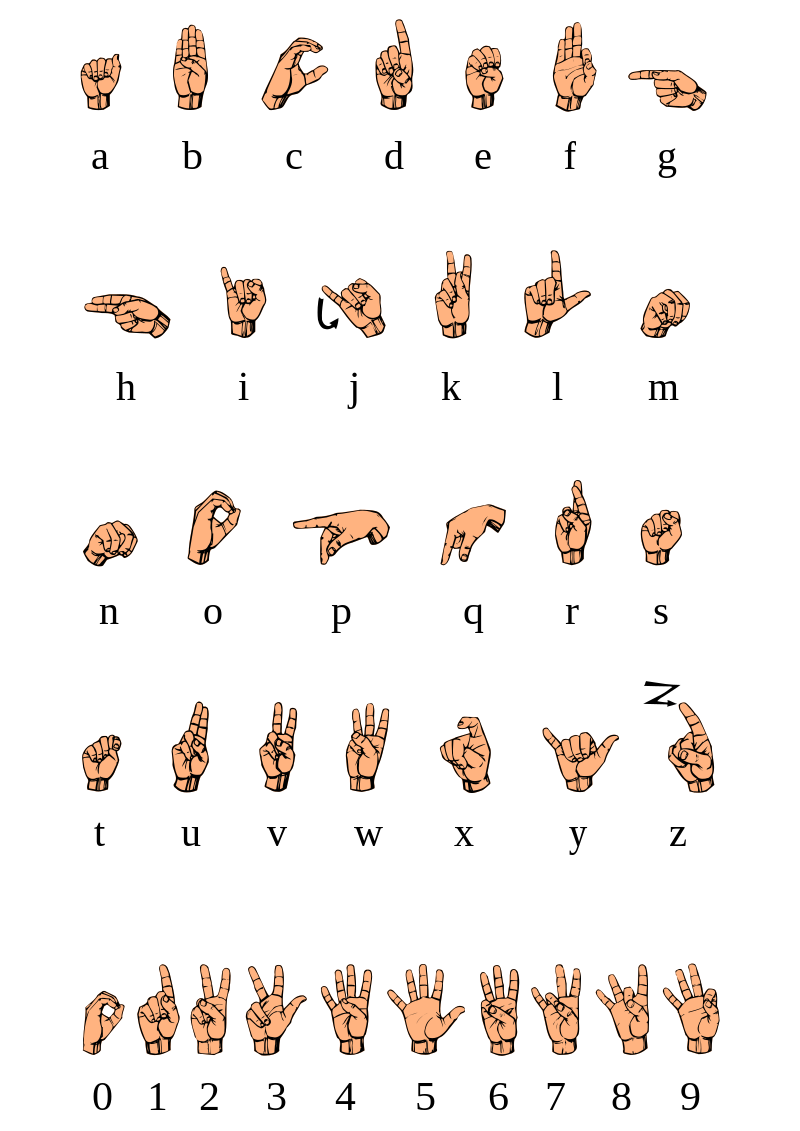
\includegraphics[scale=0.35]{ama.png}
\caption{American Manual Alphabet [Wikipedia]}
\end{figure}

W alfabecie znajduje się 26 znaków odpowiadających literom języka angielskiego. Na odpowiedniki liter składa się 19 ułożeń dłoni. Niektóre ułożenia występują kilkukrotnie tak jak litery "i" i "j" oraz "p" i "k". Różnica pomiędzy tymi znakami polega na ruchu dłonią (przy literze "j" występuje ruch w kształcie półkola) lub pozycji względem ciała (przy literze "k" dłoń jest skierowana palcami do góry, a przy literze "p" w dół lub w bok).\cite{costello}


\chapter{Konwolucyjne sieci neuronowe i rozpoznawanie obrazów}

\section{Sekcja C}
\section{Sekcja D}

\chapter{Implementacja aplikacji do rozpoznawania języka migowego ASL}

\chapter{Podsumowanie}


\listoftables{} % jeśli są tabele
\addcontentsline{toc}{chapter}{Spis tabel}

\listoffigures{} % jeśli są tabele
\addcontentsline{toc}{chapter}{Spis rysunków}

\listofcodes
\addcontentsline{toc}{chapter}{Spis listingów}

\addcontentsline{toc}{chapter}{Bibliografia}
\bibliographystyle{ieeetr}
\bibliography{bibliography/cite}


\end{document}
